
\newpage
\section{Model-Agnostic Post-hoc Methods}\label{sec:4}

\subsection{PFI - Permutation Feature Importance}

\begin{table}[H]
  \centering
  \begin{tabular}{|p{0.17\textwidth}|p{0.77\textwidth}|}
    \hline
    Form of \newline explanation & 
    Feature statistics. \\
    
    \hline
    Interpretation & 
    A feature is “important” if shuffling its values increases the model error. \\
    \hline
    Advantages &
    \begin{itemize}[nosep, left=0em]
        \item provides a highly compressed, global insight into the model’s behavior
        \item takes into account all interactions with other features
    \end{itemize} \\
    
    \hline
    Disadvantages &
    \begin{itemize}[nosep, left=0em]
        \item when the permutation is repeated, the results might vary greatly
        \item can be biased by unrealistic data instances
        \item adding a correlated feature can decrease the importance of the associated feature by splitting the importance between both features
    \end{itemize} \\
    
    \hline
    Properties & 
    post-hoc, model-agnostic, global  \\
    
    \hline
  \end{tabular}
  \caption{Overview XAI - Permutation Feature Importance.}
  \label{tab:XAIPFI}
\end{table}

Permutation Feature Importance (PFI) is a method that measures how important a feature is to the model by evaluating how the model's prediction error changes when that feature's values are randomly shuffled. The idea is that if a feature holds importance for the model, randomly rearranging its values will lead to a high increase in prediction error, which would indicate the model's dependency on the feature for accurate predictions.\\
The choice between using the training or test dataset to calculate the PFI depends on what goal you have. If you aim to measure the extent to which the model depends on a particular variable for making predictions, you should use the training data. On the other hand, if your goal is to evaluate the contribution of a feature to the model's performance on unseen data, the test data should be used. 

To compute the PFI as outlined in \cite{fisher2019all}, the process involves several steps. First, you compute the model error \( e(X) \), on the dataset \( X \). Then, for each feature, you shuffle that feature \( n \) times to create \( n \) permuted datasets \( X^p_{perm_i} \) and calculate the model error \( e(X^p_{perm_i}) \) for each permuted dataset. Finally, to derive the feature importances, you subtract these errors from the original model error: \( e(X) - e(X^p_{perm_i}) \).

Figure \ref{fig:pfi} presents a visualization of PFI using Linear Regression on training and test set of a diabetes dataset:

\begin{figure}[H]
    \centering
    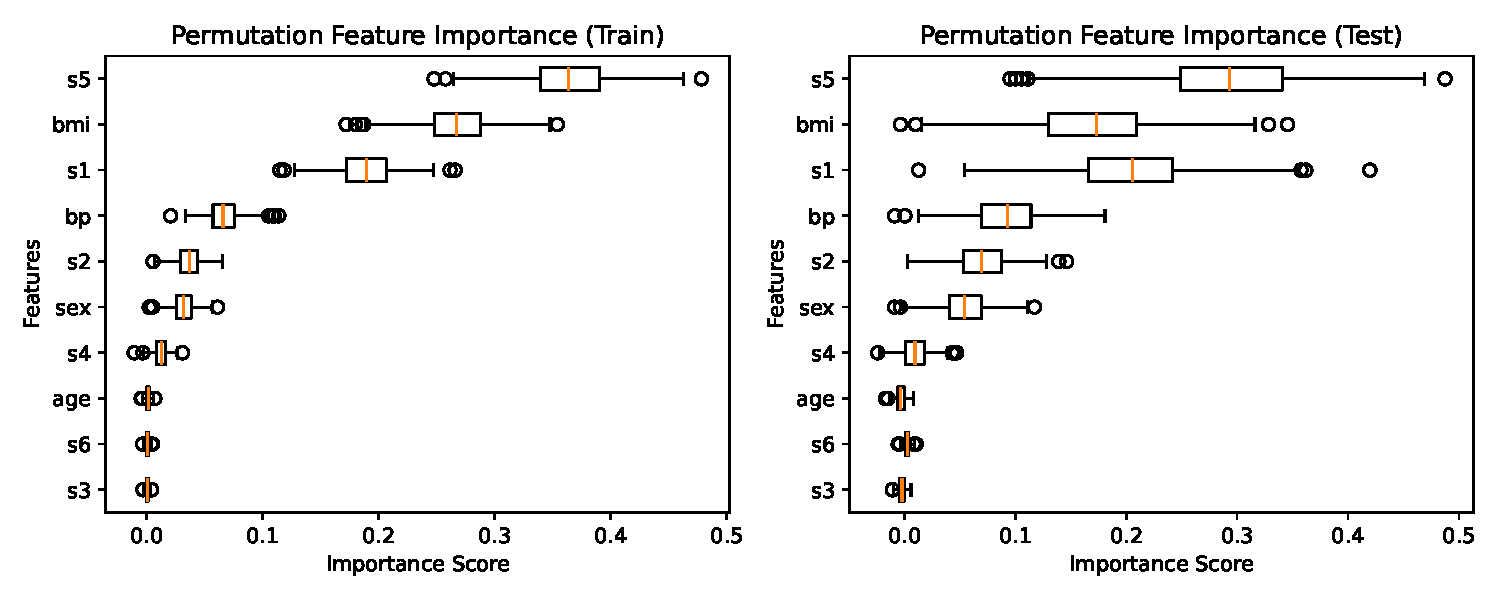
\includegraphics[width=1\linewidth]{pics/Permutation_Feature_Importance.pdf}
    \caption[Visualization of PFI using LR.]{Visualization of Permutation Feature Importance using Linear Regression on training and test set of a diabetes dataset.}
    \label{fig:pfi}
\end{figure}

The PFI calculated on the training set aligns with the weights of the Linear Regression model (Figure \ref{fig:LRW}) as expected. On the test set, the computed PFI indicates that when applying the model to new data, the feature $bmi$ is less important than feature $s_1$.

As observed, PFI provides a clear and comprehensive understanding of how the model behaves globally. Additionally, PFI considers not only the primary impact of features but also their interactions, as it disrupts these interactions when permutating individual features.\\
However, there are some drawbacks to consider. There are $n!$ ways to permute a vector. For instance, with just 100 data points, there are approximately $9.33 \times 10^{157}$ different permutation possibilities. This exponential increase in computational time forces choosing a fixed number of permutations to approximate the overall PFI. Consequently, the results may vary greatly each time PFI is repeated.
Another issue is that permuting a feature can lead to unrealistic data points, especially when two features are strongly correlated. 
Furthermore, adding a correlated feature can decrease the importance of the original correlated features by splitting the importance between them. This scenario can lead to a misleading importance ranking of features, potentially causing incorrect interpretations of a feature's relevance in the model.

\subsection{Shapley Values}

\begin{table}[H]
  \centering
  \begin{tabular}{|p{0.17\textwidth}|p{0.77\textwidth}|}
    \hline
    Form of \newline explanation & 
    Feature statistics. \\
    
    \hline
    Interpretation & 
    Given the current set of feature values, the contribution of a feature value to the difference between the actual prediction and the mean prediction is the estimated Shapley value. \\
    \hline
    Advantages &
    \begin{itemize}[nosep, left=0em]
        \item prediction is fairly distributed among the feature values
        \item has a solid theoretical foundation in game theory
        \item can be used for global model interpretations
    \end{itemize} \\
    
    \hline
    Disadvantages &
    \begin{itemize}[nosep, left=0em]
        \item requires a lot of computing time
        \item problem with correlated features, can include unrealistic data instances
        \item Shapley values can be misinterpreted
        \item no sparse explanation, always use of all the features
    \end{itemize} \\
    
    \hline
    Properties & 
    post-hoc, model-agnostic, local/global  \\
    
    \hline
  \end{tabular}
  \caption{Overview XAI - Shapley Values.}
  \label{tab:XAIShapVal}
\end{table}

Shapley values, first introduced by Shapley \cite{shapley1953value} in 1953, present a method from coalitional game theory. This approach aims to assign fair payouts to players based on their individual contributions to the overall payout within a game. When applied to machine learning, Shapley values attribute the prediction of a model to its individual features. This is achieved by considering all potential combinations of features and evaluating how the prediction changes when each feature is included.\\
A Shapley value can be expressed as follows:

\begin{equation}
    \phi_j(val)=\sum_{S\subseteq \{1,\dots ,p\}\backslash\{j\}} \overbrace{\dfrac{|S|!(p-|S|-1)!}{p!}}^{\text{Weight}} \underbrace{(val(S\cup \{j\})-val(S))}_{\text{Marginal Contribution of Feature } j \text{ to Coalition } S}.
\end{equation}

Here, $S$ represents a subset of features used in the model, $p$ indicates the total number of features, and $val$ represents the prediction for feature values within set $S$, marginalized over features not included in set $S$. \\
To illustrate this more clearly, let's apply it to a Linear Regression model: $f(x) = \beta_0 + \sum_{j=1}^p x_j\beta_j$. The contribution $\phi_j$ of the j-th feature to the prediction $\hat{f}(x)$ can be expressed as
\begin{equation}
    \phi_j(\hat{f}) = \beta_j x_j - E(\beta_j X_j).
\end{equation}
In this equation, $E(\beta_j X_j)$ represents the mean effect estimate for feature $j$. The contribution, therefore, is calculated as the difference between the effect of the feature and its average effect.\\
Summing up all Shapley values results in the predicted value for the data point $x$ minus the average predicted value:
\begin{equation}
\begin{split}
    \sum_{j=1}^p\phi_j(\hat{f})&=\sum_{j=1}^p(\beta_j x_j - E(\beta_j X_j)) = (\beta_0 + \sum_{j=1}^p\beta_j x_j) -(\beta_0 + \sum_{j=1}^p E(\beta_j X_j)) \\
    &= \hat{f}(x) - E(\hat{f}(x)).
\end{split}
\end{equation}

In Figure \ref{fig:shapley}, the Shapley values for a single prediction from a diabetes dataset are displayed:

\begin{figure}[H]
    \centering
    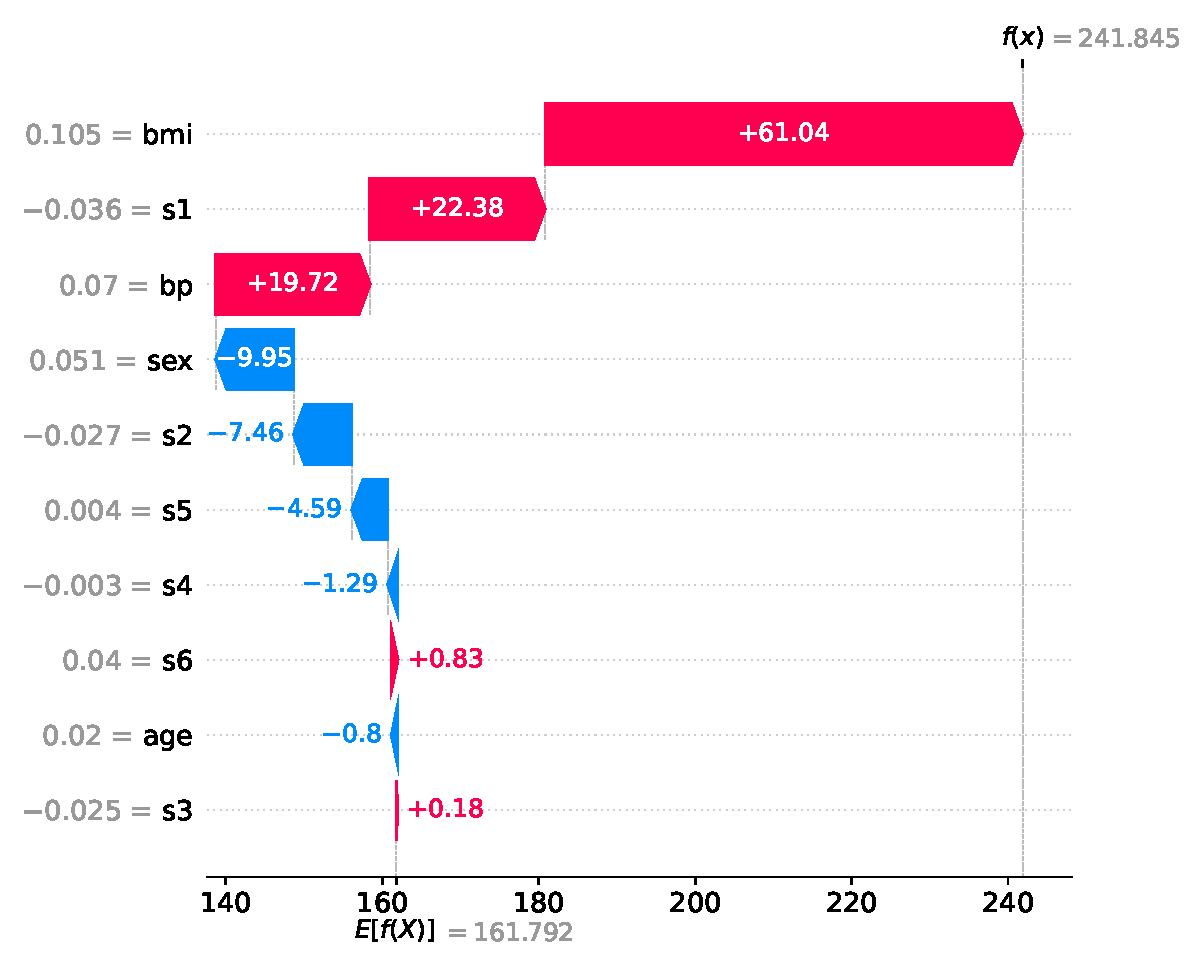
\includegraphics[width=0.8\linewidth]{pics/shap_waterfall.pdf}
    \caption[Visualizing Shapley values through a Waterfall Plot.]{Visualizing Shapley values through a Waterfall Plot with the SHAP library using Linear Regression on a test data point of a diabetes dataset.}
    \label{fig:shapley}
\end{figure}

We observe that the $bmi$ feature significantly influenced this particular prediction. However, despite the large weight of the feature $s5$ in the model, its impact appears comparatively lower than that of other features. 

Aggregating all Shapley values into a single figure can provide us with comprehensive insights into the model's global behavior, as illustrated in the following figure:

\begin{figure}[H]
    \centering
    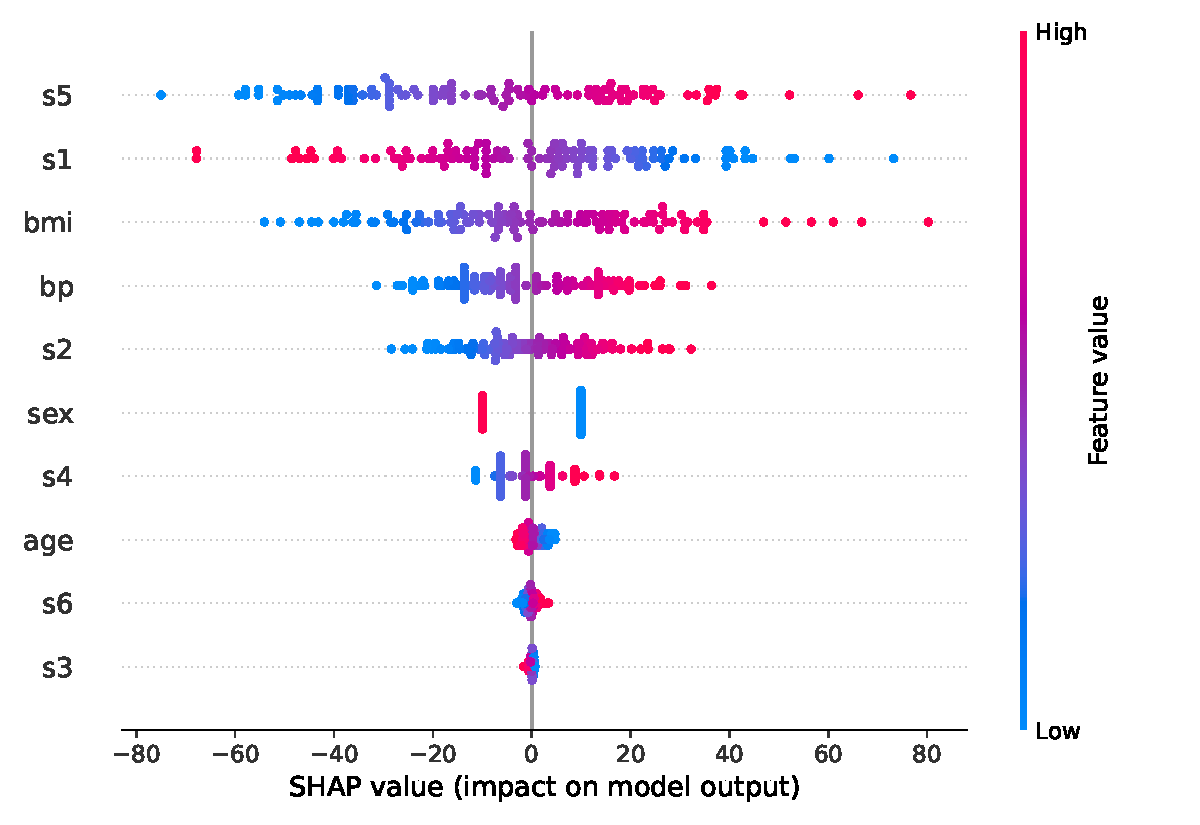
\includegraphics[width=0.8\linewidth]{pics/shap_summary_plot.pdf}
    \caption[Visualizing Shapley values through a Summary Plot]{Visualizing Shapley values through a Summary Plot with the SHAP library using Linear Regression on a test dataset of a diabetes dataset.}
    \label{fig:shapley_sum}
\end{figure}

In addition to this, various other Shapley value global interpretation methods exist, delivering feature importance values, feature dependence analysis, exploration of interactions, and clustering techniques.

The problem with Shapley values lies in their computational complexity, which grows exponentially as more features are included. This expansion occurs due to the exponential increase in possible coalitions with each additional feature. Moreover, using more complex, non-linear models further complicates the computation. In addressing this challenge \cite{vstrumbelj2014explaining} proposed an approximation technique using Monte Carlo sampling.
Additionally, \cite{lundberg2017unified} proposed the SHAP framework, which includes KernelSHAP, an alternative kernel-based estimation approach for Shapley values inspired by local surrogate models, TreeSHAP, an efficient estimation approach for tree-based models and global interpretation methods based on aggregations of Shapley values. \\
Another issue arises when dealing with correlated features, which can lead to the inclusion of unrealistic data instances. Additionally, there is a potential for misinterpretation, wherein Shapley values might be mistakenly perceived as the difference in predicted values after removing a feature from the model training. \\
A less desirable aspect of Shapley values is their inherent requirement to use all features.
